

\chapter{The Fiat Shamir Transform}

\section{Signature Schemes and Identification Schemes}
    Signature Schemes immediately yield Identification Schemes
    \begin{center}
        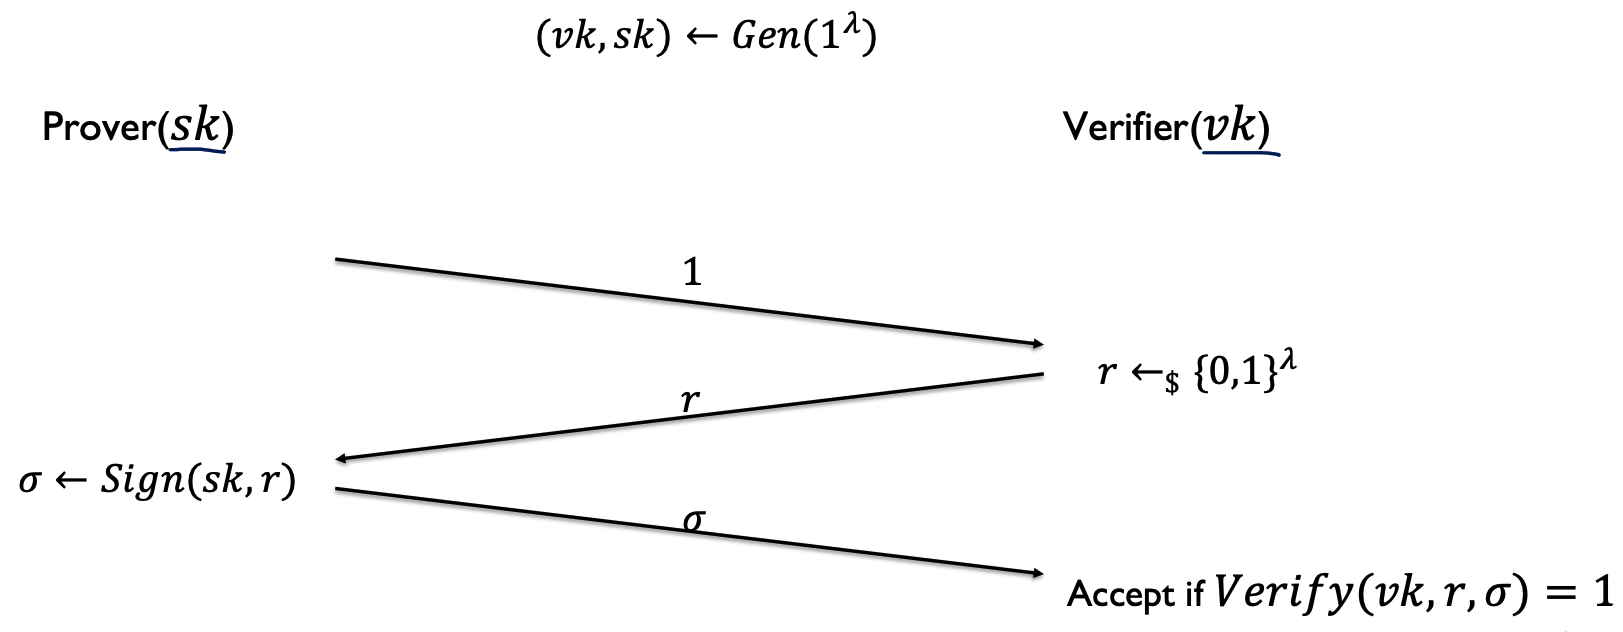
\includegraphics[width=120mm]{Graphics/Digital Signatures/fst1.png}
    \end{center}
    \begin{itemize}
        \item Signature Schemes immediately yield Identification Schemes
        \item What about the converse?
        \item Idea: Let the prover choose the challenge $r$ by himself to remove the second message
        \item Obviously insecure if prover can choose $r$ freely
        \item Idea of Fiat and Shamir: Make $r$ a function of $I$...
        \item ... and a message $m$ we want to sign
        \item This function should be unpredictable for every new $I$ and $m$
    \end{itemize}

\section{The Fiat Shamir Transform}
    \begin{itemize}
        \item Let $(Gen,P_1,P_2,V)$ be an identification scheme
        \item Let $H: \{0,1\}^* \rightarrow \Omega_{pk}$ be a hash function
        \item The Fiat-Shamir transform $(Gen',Sign',Verify')$ of $(Gen,P_1,P_2,V)$ is given as follows:
        \begin{itemize}
            \item $Gen'(1^{\lambda})$: Compute $(pk,sk) \leftarrow Gen(1^{\lambda})$.
            Output $vk \leftarrow pk$ and $sk$
            \item $Sign'(sk,m)$:
            \begin{itemize}
                \item Compute $(I,st) \leftarrow P_1(sk)$
                \item Compute $r \leftarrow H(I,m)$
                \item Compute $s \leftarrow P_2(sk,st,r)$
                \item Compute $\sigma \leftarrow (r,s)$
            \end{itemize}
            \item $Verify'(vk=pk,m,\sigma = (I,r,s))$: Let $I \leftarrow V(ppk,r,s)$\\
            If $V(pk,r,s)=I$ and $r=H(I,m)$ and output 1, otherwise 0.
        \end{itemize}
    \end{itemize}

\section{Security}
    \begin{theorem}\label{thm9.3}
        \begin{itemize}
            \item Assume that $(Gen,P_1,P_2,V)$ is a secure identification scheme
            \item Assume further that $H$ is modeled as a random oracle
            \item Then $(Gen',Sign',Verify')$ is an EUF-CMA secure signature scheme
        \end{itemize}
    \end{theorem}
    \begin{proof}
        Let $\mathcal{A}$ be a PPT adversary with non-negligible advantage $\epsilon$ against the EUF-CMA security of $(Gen',Sign',Verify')$
        $$Pr[EUF-CMA_{\mathcal{A}}=1] \geq \epsilon$$
        \begin{center}
            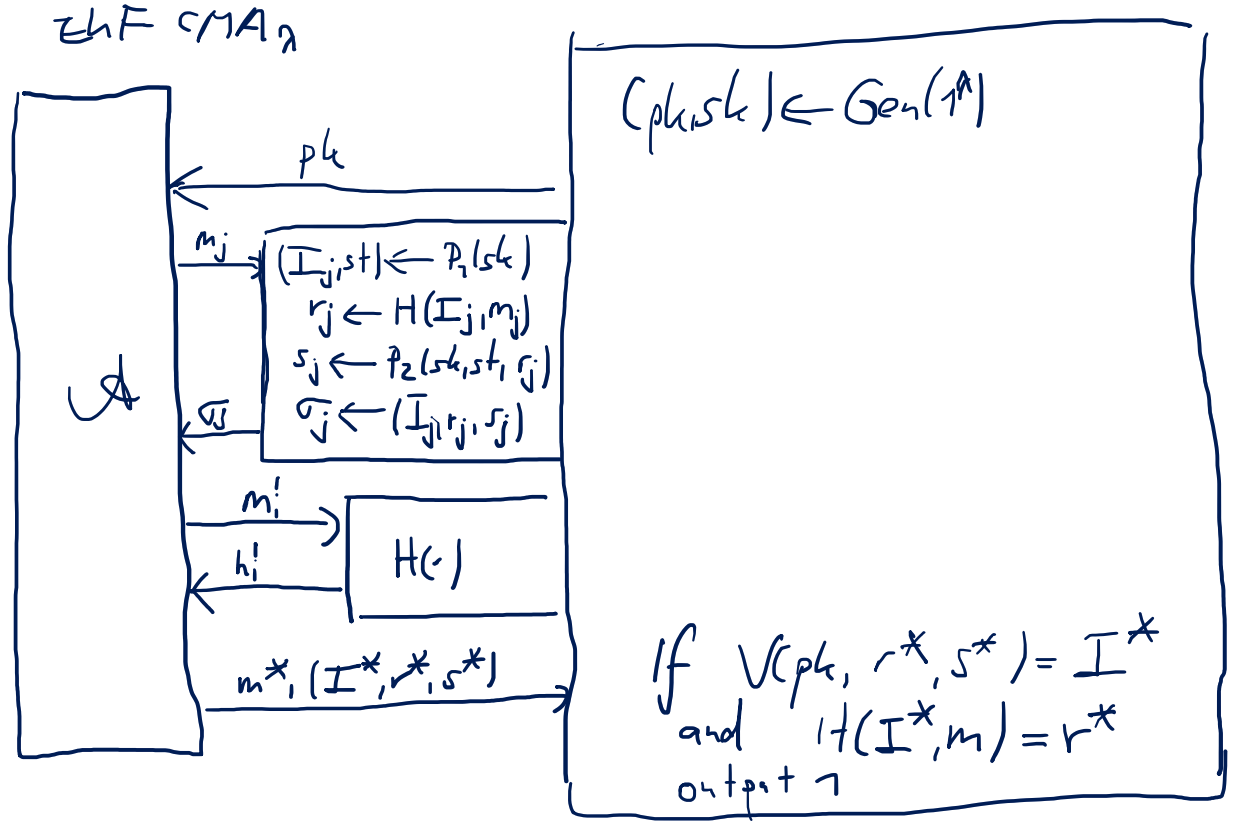
\includegraphics[width=160mm]{Graphics/Digital Signatures/fst2.png}
        \end{center}
        \begin{itemize}
            \item Assume $\mathcal{A}$ makes at most $q=poly(\lambda)$ queries to the RO $H(\cdot)$
            \item We also make the following simplifying assumptions
            \begin{itemize}
                \item $\mathcal{A}$ sends each RO-query only once
                \item We assume the RO-queries of $\mathcal{A}$ are of the form $(I'_i,m'_i)$
                \item If $\mathcal{A}$ queries the signing oracle with a message $m_j$ and obtains a signature $\sigma_j = (I_j,r_j,s_j)$, 
                then it will not query the RO $H(\cdot)$ on $(I_j,m_j)$
            \end{itemize}
        \end{itemize}
        We will now construct an adversary $\mathcal{A}$' which breaks security of $(Gen,P_1,P_2,V)$ with probability $\frac{\epsilon}{q}$
        \begin{center}
            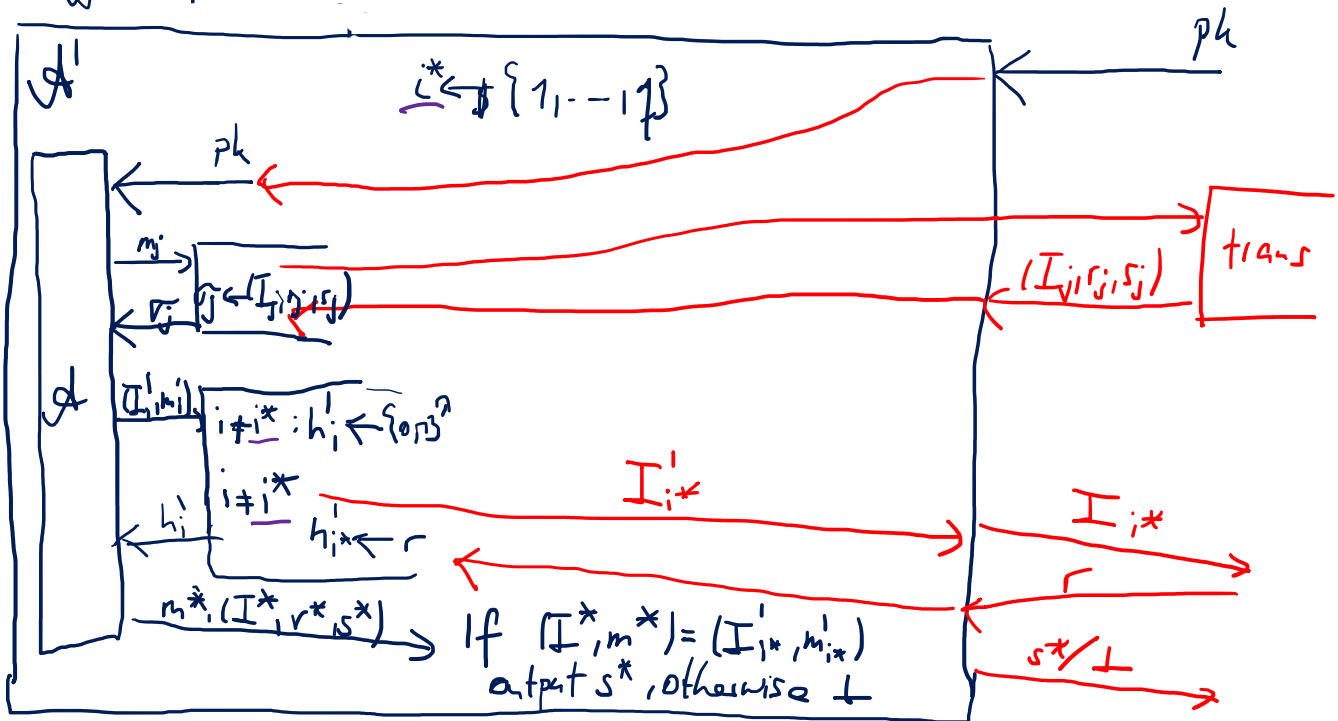
\includegraphics[width=160mm]{Graphics/Digital Signatures/fst3.png}
        \end{center}
        From the view of $\mathcal{A}$, $\mathcal{A}$' simulates the EUF-CMA experiment faithfully:
        \begin{itemize}
            \item Signing oracle simulated faithfully as the $r_j$ are chosen uniformly random
            \item Same for outputs of $H(\cdot)$
        \end{itemize}
        As in the proof of \cref{thm9.1} we can define an event $QUERIED$ by $\exists \brac{i} \in \{1,...,q\}$ s.t. $(I^*,m^*) = (I'_{\brac{i}},m'_{\brac{i}})$
        and argue that 
        $$Pr[EUF-CMA_{\mathcal{A}}=1 \wedge QUERIED] \geq \epsilon'$$
        which is non-negligible. We can conclude
        \begin{align*}
            Pr[Ident_{\mathcal{A}'}(\lambda)=1] &\geq Pr[EUF-CMA_{\mathcal{A}}(\lambda)=1 \wedge QUERIED \wedge i^*=\brac{i}]\\
            &= \underbrace{Pr[EUF-CMA_{\mathcal{A}}(\lambda)=1 \wedge QUERIED]}_{\geq \epsilon} \cdot \underbrace{Pr[i^*=\brac{i}]}_{= \frac{1}{q}}\\
            &\geq \frac{\epsilon}{q}\ \ \ \text{which is non-negligible!}
        \end{align*}
        $\Rightarrow$ This contradicts security of $(Gen,P_1,P_2,V)$
    \end{proof}
    
\section{The Schnorr Signature Scheme}
    \begin{itemize}
        \item Combining the Schnorr Identification Scheme with \cref{thm9.3} yields the following EUF-CMA secure Signature Scheme
        \item Let $\mathbb{G}$ be a cryptographic group of order $p$ with generator $g$
        \item Let $H: \{0,1\}^* \rightarrow \mathbb{Z}_p$ be a hash function
        \item The Schnorr signature scheme $(Gen,Sign,Verify)$ is given as follows
        \begin{itemize}
            \item $Gen(1^{\lambda})$: Choose $x \leftarrow_{\$} \mathbb{Z}_p$, compute $y \leftarrow_{\$} g^x$, output $vk \leftarrow y$ and $sk \leftarrow x$
            \item $Sign(sk=x,m)$: Choose $k \leftarrow_{\$} \mathbb{Z}_p$, compute $I \leftarrow g^k$, $r \leftarrow H(I,m)$, $s \leftarrow r \cdot x + k\ mod\ p$
            and output $\sigma \leftarrow (r,s)$
            \item $Verify(vk=y,m,\sigma = (r,s))$: Compute $I \leftarrow g^s \cdot y^{-r}$, if $r=H(I,m)$ output 1, otherwise 0
        \end{itemize}
    \end{itemize}

    \section{Schnorr Signatures}
        \begin{itemize}
            \item Schnorr signatures are basically the most efficient and shortest signatures when instantiated with elliptic curve groups
            \item In practice the group $\mathbb{G}$, its order $p$ and a generator $g$ are publicly fixed, e.g Ed25519
            \item Size of verification and signing keys: 256 bits (32 bytes)
            \item Size of signatures 512 bits (64 bytes)
            \item Signing: 1 exponentiation
            \item Verifying: 2 exponentiations
            \item Why are Schnorr signatures not widely used?
            \item Intellectual Property Rights!
            \item https://patents.google.com/patent/US4995082
        \end{itemize}
        \begin{center}
            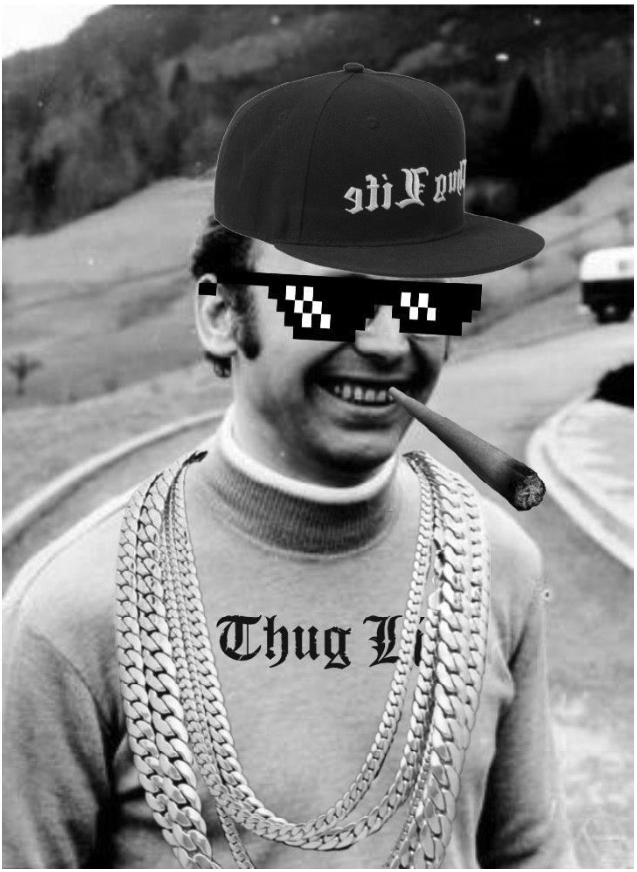
\includegraphics[width=120mm]{Graphics/Digital Signatures/fst4.png}
        \end{center}

\section{The Digital Signature Algorithm (DSA)}
    \begin{itemize}
        \item Let $\mathbb{G}$ be a cryptographic group of order $p$ with generator $g$
        \item Let $F,H: \{0,1\}^* \rightarrow \mathbb{Z}_p$ be two hash functions
        \item The DSA scheme $(Gen,Sign,Verify)$ is given as follows
        \begin{itemize}
            \item $Gen(1^{\lambda})$: Choose $x \leftarrow_{\$} \mathbb{Z}_p$, compute $y \leftarrow_{\$} g^x$, output $vk \leftarrow y$ and $sk \leftarrow x$
            \item $Sign(sk=x,m)$: Choose $k \leftarrow_{\$} \mathbb{Z}_p$, compute $r \leftarrow F(g^k)$, $s \leftarrow k^{-1} \cdot (H(m)+xr)\ mod\ p$, restart if $r=0$ or $s=0$.
            Output $\sigma \leftarrow (r,s)$
            \item $Verify(vk=y,m,\sigma = (r,s))$: If $r,s \neq 0$ and $r \leftarrow F(g^{H(m)s^{-1}}y^{rs^{-1}})$ output 1, otherwise 0
        \end{itemize}
    \end{itemize}

\section{Summary}
    \begin{itemize}
        \item Signature schemes immediately imply identification schemes
        \item Conversely, every 3-round identification scheme can be transformed into a signature scheme via the Fiat Shamir transform
        \item The security proof is in the random oracle model
        \item Using the Fiat-Shamir transform, the Schnorr identification scheme yields the currently most efficient know signature scheme with the shortest signatures
        \item Due to patent issues the slightly more contrived DSA scheme was standardized
    \end{itemize}
        

